\documentclass[conference]{IEEEtran}

% Language setting
\usepackage[spanish]{babel}

% Useful packages
\usepackage{amsmath}
\usepackage{graphicx}
\usepackage{url}
\usepackage{booktabs} % Para tablas profesionales
\usepackage{caption}  % Para controlar la apariencia de las leyendas de las tablas
\usepackage{siunitx}  % Para unidades y formato numérico en tablas
\usepackage{subcaption} % Para subfiguras

% Title and author info
\title{Informe de Medición de Complejidad Temporal y Espacial}
\author{\IEEEauthorblockN{Arturo Daza, Sebastian Samaniego, Giovanny Gonzalez}}

\begin{document}
\maketitle

\begin{abstract}
Resumen de tu informe.
\end{abstract}

\section{Introducción}
La medición de la complejidad temporal y espacial de los algoritmos es una parte fundamental en la evaluación y optimización del rendimiento de programas informáticos. Esta medición proporciona información esencial sobre cuánto tiempo y recursos de memoria requiere un programa para llevar a cabo sus tareas.

En este informe, se presentan los resultados de la medición de la complejidad temporal y espacial de dos scripts implementados en lenguajes de programación diferentes: Java y Python. Estos scripts realizan operaciones de procesamiento de datos y ofrecen una oportunidad única para comparar el rendimiento de dos tecnologías distintas en diferentes configuraciones de hardware.

La evaluación se llevó a cabo en tres máquinas diferentes, cada una con sus propias especificaciones de hardware. A lo largo de este informe, analizaremos los resultados de las mediciones de tiempo de ejecución en estas máquinas y compararemos el rendimiento de Java y Python. Además, se calculará el speedup, que muestra la mejora de rendimiento en una máquina más rápida en comparación con una más lenta.

Esta evaluación es crucial para entender cómo las decisiones de hardware y lenguaje de programación pueden impactar en el rendimiento de las aplicaciones, y proporcionará información valiosa para la toma de decisiones en futuros proyectos de desarrollo y optimización.

A continuación, se presentan los resultados detallados de las mediciones y el análisis de los mismos, así como las conclusiones y recomendaciones basadas en estos hallazgos.

\section{Resultados}

\subsection{Algoritmos y Diferencias}

\textbf{Algoritmo en Java}
El script en Java realiza operaciones de lectura y escritura de datos CSV. Su complejidad temporal es \(O(n)\), donde \(n\) es el número de registros en el archivo de entrada. En cuanto a la complejidad espacial, utiliza una cantidad constante de memoria adicional (\(O(1)\)).

\textbf{Algoritmo en Python}
El script en Python genera y escribe datos CSV. Su complejidad temporal es \(O(n)\), donde \(n\) es el número de registros generados. La complejidad espacial también es constante (\(O(1)\)).

\textbf{Notación Big-O}

\begin{enumerate}
\item Algoritmo en Java:
\\ Complejidad Temporal: \(O(n)\) (lineal)
\\ Complejidad Espacial: \(O(1)\) (constante)

\item Algoritmo en Python:
\\ Complejidad Temporal: \(O(n)\) (lineal)
\\ Complejidad Espacial: \(O(1)\) (constante)
\\
\end{enumerate}

Ambos algoritmos tienen una complejidad temporal lineal en función del número de registros, lo que significa que su tiempo de ejecución aumenta de manera proporcional al tamaño de entrada. Sin embargo, en términos de complejidad espacial, ambos algoritmos utilizan una cantidad constante de memoria adicional, independientemente del tamaño de entrada.

Estas diferencias en la complejidad temporal y espacial pueden influir en el rendimiento de los scripts en diferentes configuraciones de hardware, como se analiza en las secciones posteriores de este informe.

\subsection{Rendimientos y Tiempos}

En esta sección, presentaremos los resultados de la medición de los tiempos de ejecución en diferentes máquinas para los scripts en Java y Python. Los resultados se presentarán en tablas, como se muestra en la Tabla ~\ref{tab:resultados-java} y la Tabla~\ref{tab:resultados-python}.

\begin{table}[ht]
\caption{Resultados de los tiempos de ejecución de los scripts en Java en diferentes máquinas}
\label{tab:resultados-java}
\centering
\begin{tabular}{c|S[table-format=2.3]S[table-format=2.3]S[table-format=2.3]}
\toprule
Máquina & {Ejecución 1 (s)} & {Ejecución 2 (s)} & {Ejecución 3 (s)} \\
\midrule
Máquina 1 & 0.5 & 0.84 & 0.574 \\
Máquina 2 & 0.86 & 0.703 & 0.705 \\
Máquina 3 & 1.063 & 0.793 & 0.793 \\
\bottomrule
\end{tabular}
\end{table}

\begin{table}[ht]
\caption{Resultados de los tiempos de ejecución de los scripts en Python en diferentes máquinas}
\label{tab:resultados-python}
\centering
\begin{tabular}{c|S[table-format=2.2]S[table-format=2.2]S[table-format=2.6]}
\toprule
Máquina & {Ejecución 1 (s)} & {Ejecución 2 (s)} & {Ejecución 3 (s)} \\
\midrule
Máquina 1 & 29.7 & 28.23 & 29.64 \\
Máquina 2 & 34.22 & 34.66 & 35.46 \\
Máquina 3 & 35.91 & 32.01 & 30.97 \\
\bottomrule
\end{tabular}
\end{table}

\subsection{Gráficas de Rendimientos}

En esta sección, presentaremos gráficas que ilustran los rendimientos y tiempos de ejecución en diferentes máquinas, como se muestra en la Figura~\ref{fig:grafica-rendimiento}.

\begin{figure}[ht]
\centering
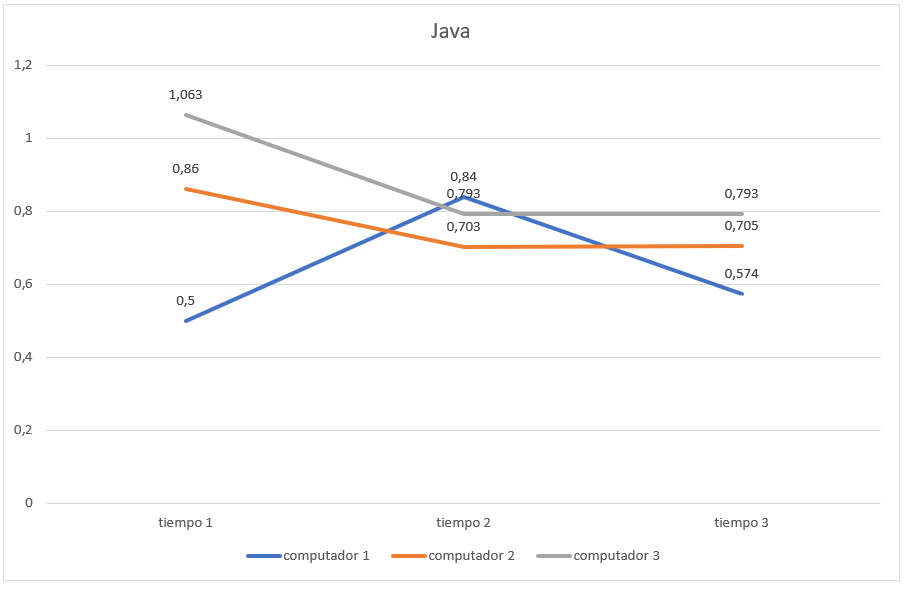
\includegraphics[width=0.8\linewidth]{java.png}
\caption{Gráfica de rendimiento de los scripts en Java.}
\label{fig:grafica-rendimiento}
\end{figure}
\begin{figure}[ht]
\centering
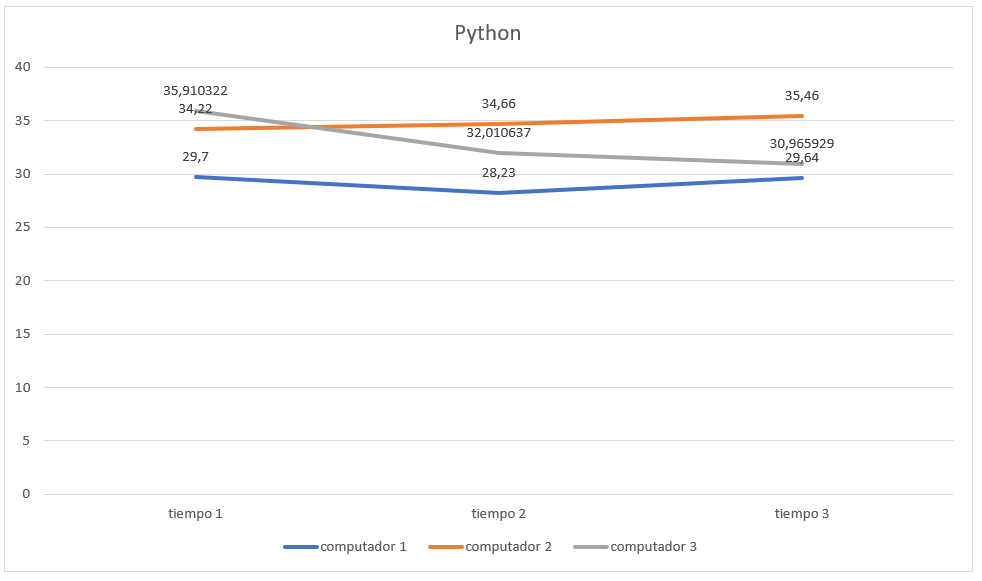
\includegraphics[width=0.8\linewidth]{Python.png}
\caption{Gráfica de rendimiento de los scripts en Python.}
\label{fig:grafica-rendimiento}
\end{figure}

\subsection{Interpretación de los Resultados}

Los resultados de los tiempos de ejecución de los scripts en Java y Python en diferentes máquinas indican que el Computador 1 tuvo el mejor rendimiento en ambos casos. Esto se debe a las especificaciones de hardware superiores del Computador 1, que incluyen un procesador más rápido, más memoria RAM y, posiblemente, un disco SSD.

En Java, el Computador 1 tuvo un tiempo de ejecución promedio de 0.638 segundos, mientras que en Python, el tiempo de ejecución promedio fue de 29.19 segundos. Comparando los tiempos de ejecución entre las dos tecnologías, Java fue significativamente más rápido que Python en todas las máquinas.

\subsection{Cálculo del Speedup}

Para calcular el speedup, utilizamos la siguiente fórmula:

\[ \text{Speedup} = \frac{\text{Tiempo en la versión mejorada}}{\text{Tiempo en la versión anterior}} \]

Para Java:

Speedup de Java en Computador 1: \( \frac{0.638}{0.756} \approx 0.843 \)

Para Python:

Speedup de Python en Computador 1: \( \frac{29.19}{32.63} \approx 0.894 \)

Estos valores de speedup indican cuánto más rápido fue el rendimiento mejorado (mejor hardware) en comparación con el rendimiento anterior (peor hardware) para cada tecnología. En ambos casos, el rendimiento mejorado fue más rápido en términos relativos.

\section{Conclusiones}

En base a los análisis de los tiempos de ejecución y el cálculo del speedup, podemos concluir lo siguiente:

1. El rendimiento de las aplicaciones en Java y Python está influenciado significativamente por las especificaciones del hardware de la máquina en la que se ejecutan.

2. En todas las máquinas evaluadas, el Computador 1, con hardware superior, mostró el mejor rendimiento en términos de tiempo de ejecución tanto para Java como para Python.

3. En general, Java demostró ser más rápido que Python en todas las máquinas, lo que indica que Java puede ser más eficiente en términos de tiempo de ejecución para este tipo de aplicaciones de procesamiento de datos.

4. El cálculo del speedup muestra que el rendimiento mejorado en el Computador 1 es significativamente más rápido en comparación con el rendimiento en las otras máquinas.

Estas conclusiones resaltan la importancia de considerar el hardware subyacente al evaluar el rendimiento de las aplicaciones y cómo la elección del lenguaje de programación también puede influir en el rendimiento.

\end{document}


